\documentclass[11pt, a4paper, oneside]{ctexbook}
\usepackage{amsmath, amsthm, amssymb, bm, graphicx, hyperref, mathrsfs, enumitem, geometry, listings, xcolor}
\title{{\Huge{\textbf{《中南大学\ 软件测试工程》}}}\\课后作业四}
\author{徐鸣飞}
\date{2023 年 11 月 30 日}
\linespread{1.5}

\newtheorem{theorem}{定理}[section]
\newtheorem{definition}[theorem]{定义}
\newtheorem{lemma}[theorem]{引理}
\newtheorem{corollary}[theorem]{推论}
\newtheorem{example}[theorem]{例}
\newtheorem{proposition}[theorem]{命题}

\geometry{a4paper,scale=0.7}


\begin{document}

\maketitle
\pagenumbering{roman}
\setcounter{page}{1}
\newpage
\pagenumbering{Roman}
\setcounter{page}{1}
\tableofcontents
\newpage
\setcounter{page}{1}
\pagenumbering{arabic}

\chapter{订单处理系统}
\section{0层DFD图}
\centering
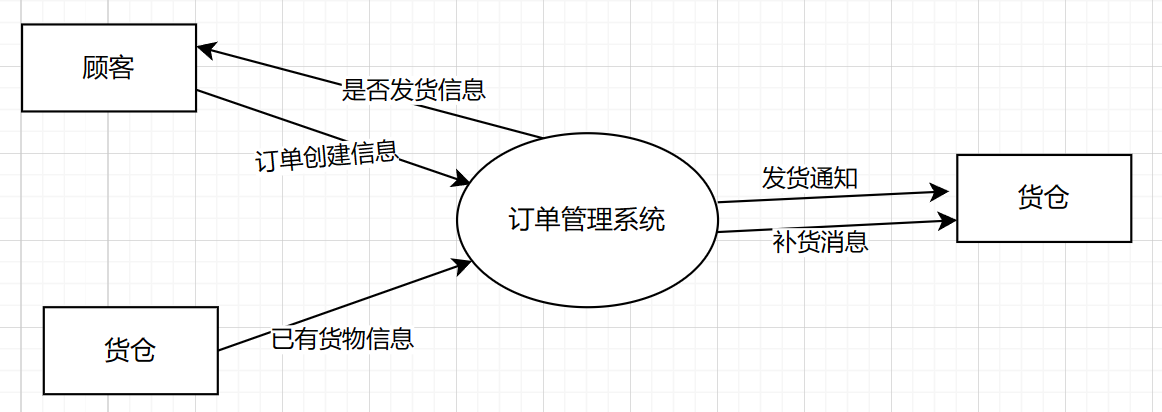
\includegraphics[width=\textwidth]{1.png}
\label{fig:DFD0}

\newpage
\section{1层DFD图}
\centering
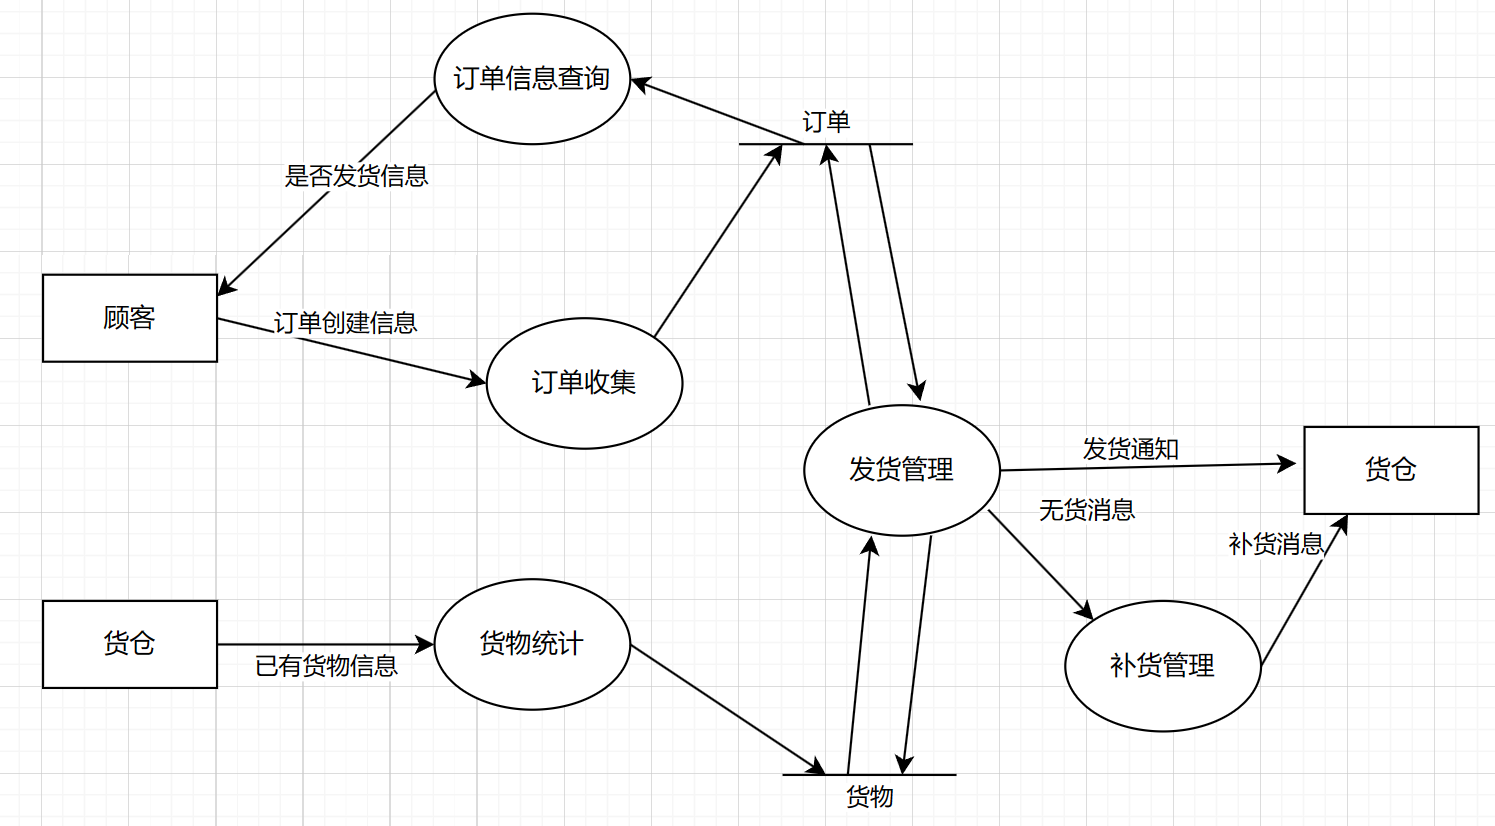
\includegraphics[width=\textwidth]{2.png}
\label{fig:DFD1}

\newpage
\section{实体关系图及数据对象、关系、属性}
\centering
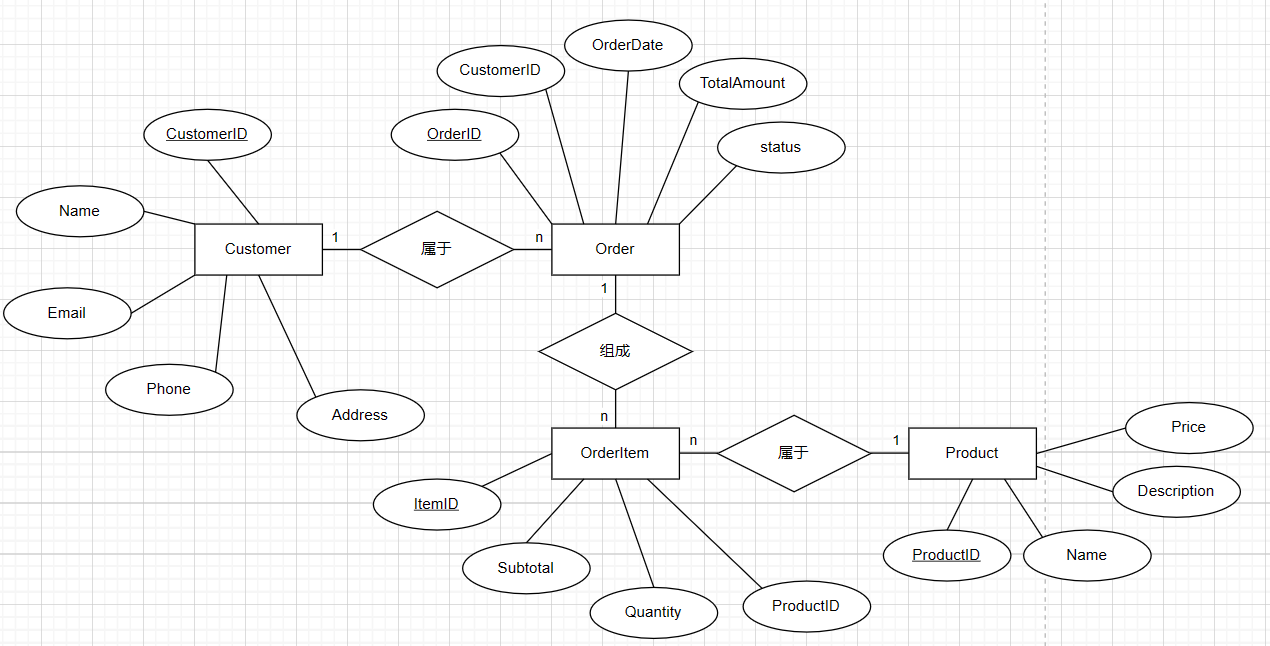
\includegraphics[width=\textwidth]{3.png}
\label{fig:ER}
\raggedright
关系说明:
\begin{itemize}
    \item \textbf{Customer与Order(一对多关系)}:一个顾客可以有多个订单,但一个订单只属于一个顾客。
    \item \textbf{Order与OrderItem(一对多关系)}:一个订单可以包含多个订单项(多种产品),但一个订单项只属于一个订单。
    \item \textbf{Product与OrderItem(一对多关系)}:一个产品可以包含在多个订单项中,一个订单项对应一个产品。
\end{itemize}
\newpage

\section{Order的状态转换图}
\centering
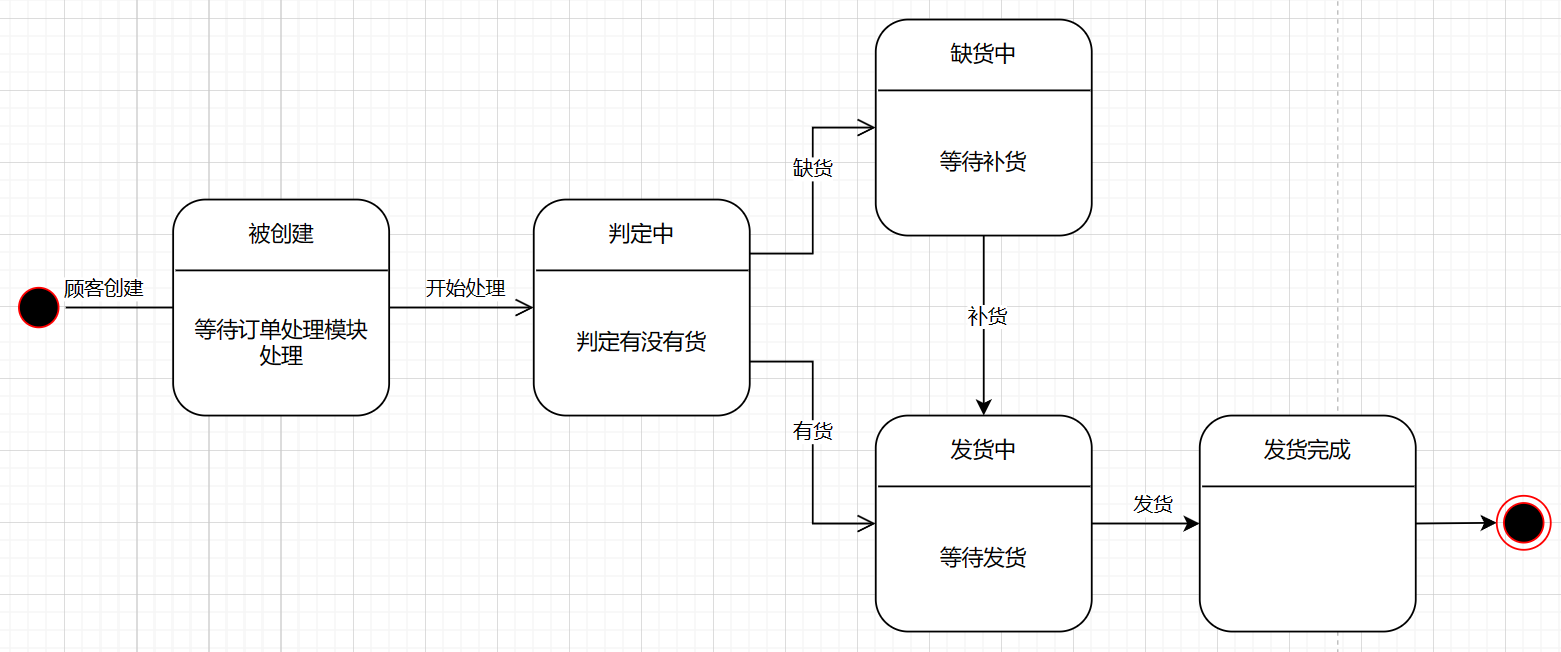
\includegraphics[width=\textwidth]{4.png}
\label{fig:status}
\end{document}